\documentclass[12pt, twoside]{article}
\usepackage[letterpaper, margin=1in, headsep=0.5in]{geometry}
\usepackage[english]{babel}
\usepackage[utf8]{inputenc}
\usepackage{amsmath}
\usepackage{amsfonts}
\usepackage{amssymb}
\usepackage{tikz}
\usetikzlibrary{quotes, angles}
\usepackage{graphicx}
\usepackage{enumitem}
\usepackage{multicol}

\newif\ifmeta
\metatrue %print standards and topics tags

\title{Regents Geometry}
\author{Chris Huson}
\date{September 2020}

\usepackage{fancyhdr}
\pagestyle{fancy}
\fancyhf{}
\renewcommand{\headrulewidth}{0pt} % disable the underline of the header
\raggedbottom


\fancyhead[LE]{\thepage}
\fancyhead[RO]{\thepage \\ Name: \hspace{4cm} \,\\}
\fancyhead[LO]{BECA / Dr. Huson / Geometry \\* 1-12 Test angles}

\begin{document}

\subsubsection*{Test: I can solve for angle measures}
\emph{Diagrams are not necessarily drawn to scale unless otherwise stated.}
\begin{enumerate}
\item I have my own calculator with me today. (circle one). Yes \qquad No
\item I have a notebook, ruler, and protractor (circle one). Yes \qquad No \vspace{0.5cm}
  
\item Given $\overline{ABC}$, $AB=29$, and $BC=63$. 
  Find ${AC}$.
  \begin{flushright}
    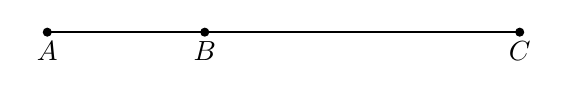
\begin{tikzpicture}
      \draw [-, thick] (0,0)--(6,0);
      \draw [fill] (0,0) circle [radius=0.05] node[below]{$A$};
      \draw [fill] (2,0) circle [radius=0.05] node[below]{$B$};
      \draw [fill] (6,0) circle [radius=0.05] node[below]{$C$};
    \end{tikzpicture} \vspace{2cm}
  \end{flushright}

\item Given $\overline{DEF}$, $DE=5 \frac{1}{14}$, and $DF=9 \frac{4}{7}$.
  Find ${EF}$. State as a fraction. \vspace{1cm}
  \begin{flushright}
    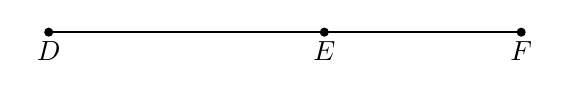
\begin{tikzpicture}
      \draw [-, thick] (0,0)--(6,0);
      \draw [fill] (0,0) circle [radius=0.05] node[below]{$D$};
      \draw [fill] (3.5,0) circle [radius=0.05] node[below]{$E$};
      \draw [fill] (6,0) circle [radius=0.05] node[below]{$F$};
    \end{tikzpicture} \vspace{1cm}
  \end{flushright}

\item Find the distance between $M$ and $N$. 
\begin{flushright}
    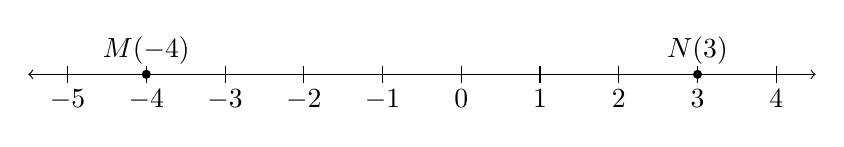
\begin{tikzpicture}
      \draw [<->] (-5.5,0)--(4.5,0);
      \foreach \x in {-5,...,4}
        \draw[shift={(\x,0)},color=black] (0pt,-3pt) -- (0pt,3pt) node[below=5pt]  {$\x$};
        \draw [fill] (-4,0) circle [radius=0.05] node[above] {$M(-4)$};
        \draw [fill] (3,0) circle [radius=0.05] node[above] {$N(3)$};
    \end{tikzpicture}
  \end{flushright} \vspace{0.75cm}  

\item Find $GH$, given $G=1.4$ and $H=6.1$.
\begin{flushright}
  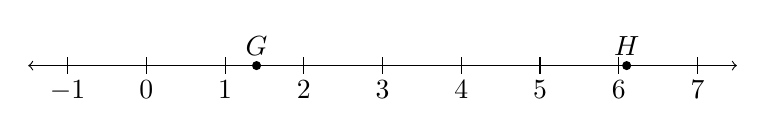
\begin{tikzpicture}
    \draw [<->] (-1.5,0)--(7.5,0);
    \foreach \x in {-1,...,7} %2 leading for diff!=1
      \draw[shift={(\x,0)},color=black] (0pt,-3pt) -- (0pt,3pt) node[below=5pt]  {$\x$};
      \draw [fill] (1.4,0) circle [radius=0.05] node[above] {$G$};
      \draw [fill] (6.1,0) circle [radius=0.05] node[above] {$H$};
  \end{tikzpicture}
\end{flushright} \vspace{1.75cm}

\item Draw the ray $\overrightarrow{ST}$ with a straight edge (or ruler). Measure $ST$ in centimeters.\\
  \vspace{0.5cm}
  \begin{center}
    \begin{tikzpicture}
    \draw [fill] (0,0) circle [radius=0.05] node[below]{$T$};
    \draw [fill] (10:7) circle [radius=0.05] node[below]{$S$};
  \end{tikzpicture}
  \end{center}

\newpage
\item Two rays with a common vertex compose a(n) $\rule{4cm}{0.15mm}$. \bigskip
\item Points that are all located on the same line are $\rule{4cm}{0.15mm}$.\bigskip

\item Use conventional notation to write the names of the ray, line, and segment shown.\\.\\
  \vspace{0.5cm}
  \begin{tikzpicture}
    \draw [-, thick] (1,0)--(4,2);
    \draw [fill] (1,0) circle [radius=0.05] node[below]{$A$};
    \draw [fill] (4,2) circle [radius=0.05] node[above left]{$B$};
    \node at (0,0) {(a)};
  \end{tikzpicture} \hspace{.25cm}
  \begin{tikzpicture}
    \draw [->, thick] (0,0)--(3,1.5);
    \draw [fill] (0,0) circle [radius=0.05] node[below]{$P$};
    \draw [fill] (2,1) circle [radius=0.05] node[below]{$Q$};
    \node at (-1,0) {(b)};
  \end{tikzpicture}  \hspace{.1cm}
  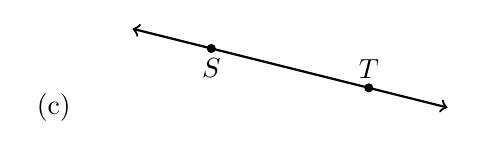
\begin{tikzpicture}
    \draw [<->, thick] (1,1)--(5,0);
    \draw [fill] (2,0.75) circle [radius=0.05] node[below]{$S$};
    \draw [fill] (4,.25) circle [radius=0.05] node[above]{$T$};
    \node at (0,0) {(c)};
  \end{tikzpicture}

  \vspace{1cm}

\item Two line segments or angles of equal measure are $\rule{4cm}{0.15mm}$. \bigskip

\item Identify two line segments in the given plane.\\[0.25in]
  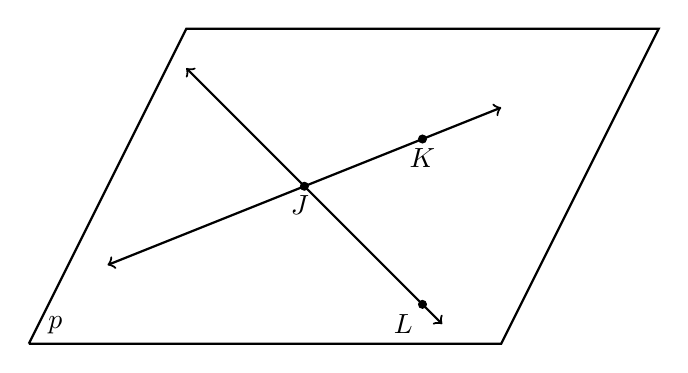
\begin{tikzpicture}
    \draw [thick](0,0) node[above right]{$\ p$} --(6,0)--(8,4)--(2,4)--(0,0);
    \draw [<->, thick] (1,1)--(6,3);
    \draw [fill] (3.5,2) circle [radius=0.05] node[below]{$J \ $};
    \draw [fill] (5,2.6) circle [radius=0.05] node[below]{$K$};
    \draw [<->, thick] (2,3.5)--(5.25,.25);
    \draw [fill] (5,0.5) circle [radius=0.05] node[below left]{$L$};
  \end{tikzpicture} \vspace{1cm}

  \item Given isosceles $\triangle XYZ$ with $\overline{XY} \cong \overline{XZ}$. On the diagram mark the congruent line segments with tick marks.
  \begin{center}
  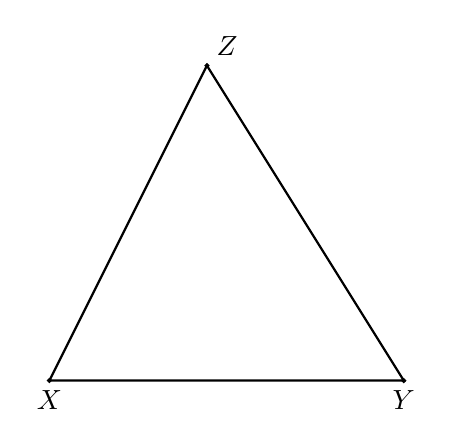
\begin{tikzpicture}[scale=0.5]
    \draw [thick](0,0)--(9,0)--(4,8)--(0,0);
    \draw [fill] (0,0) circle [radius=0.05] node[below]{$X$};
    \draw [fill] (9,0) circle [radius=0.05] node[below]{$Y$};
    \draw [fill] (4,8) circle [radius=0.05] node[above right]{$Z$};
  \end{tikzpicture}
  \end{center}

\newpage
\item Given the situation in the diagram, answer each question. Circle True or False. 
  \vspace{0.25cm}
      \begin{multicols}{2}
        \begin{enumerate}
          \item T or F: $\overrightarrow{PR}$ and $\overrightarrow{PU}$ are opposite rays.\bigskip
          \item T or F: $\angle TPR$ is an obtuse angle.\bigskip
          \item T or F: $\angle RPS$ and $\angle TPU$ are \\adjacent angles. \bigskip
        \end{enumerate}
      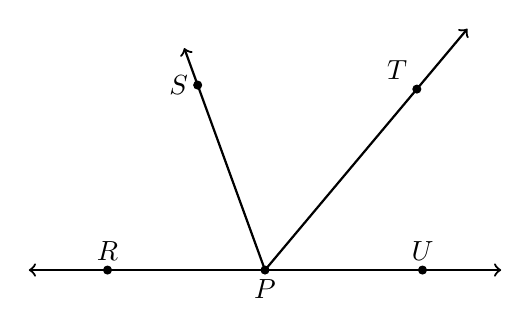
\begin{tikzpicture}[scale=1]
        \draw [->, thick] (0,0)--(50:4);
        \draw [<->, thick] (-3,0)--(3,0);
        \draw [->, thick] (0,0)--(110:3);
        \draw [fill] (110:2.5) circle [radius=0.05] node[left ]{$S$};
        \draw [fill] (50:3) circle [radius=0.05] node[above left ]{$T$};
        \draw [fill] (0,0) circle [radius=0.05] node[below]{$P$};
        \draw [fill] (2,0) circle [radius=0.05] node[above]{$U$};
        \draw [fill] (-2,0) circle [radius=0.05] node[above]{$R$};
      \end{tikzpicture}
      \end{multicols}

\item As shown below, two lines intersect making four angles: $\angle 1$, $\angle 2$, $\angle 3$, and $\angle 4$.
  \begin{center}
  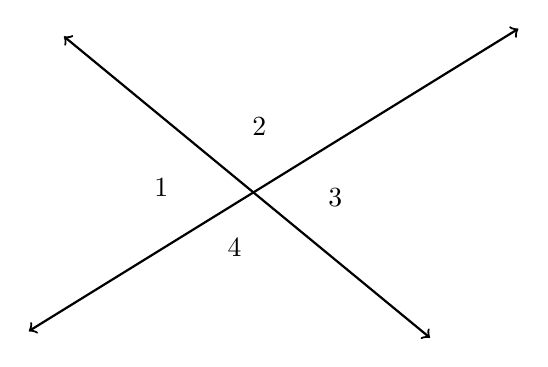
\begin{tikzpicture}[scale=0.7, rotate=15]
    \draw [<->, thick] (0,-1.5)--(10,1.5);
    \draw [<->, thick] (2,3.5)--(7,-3.5);
    \node at (3,.4){1};
    \node at (6,-.6){3};
    \node at (5,1){2};
    \node at (4,-1){4};
  \end{tikzpicture}
  \end{center}
  \begin{enumerate}
  \item Given that $m\angle 1= 75^\circ$, find $m\angle 2=$ \rule{2.5cm}{0.15mm} \bigskip
  \item Find $m\angle 3=$ \rule{2.5cm}{0.15mm} \bigskip
  \item True or false, $\angle 1$ and $\angle 4$ are supplementary angles. \rule{3cm}{0.15mm}
\end{enumerate}

\item 
  \begin{enumerate}
    \item Given, the diagram below. Name a right angle:  \rule{4cm}{0.15mm}  \bigskip
    \item Name the angle that is opposite to $\angle AOB$: \rule{4cm}{0.15mm}  \bigskip
    \item Name an angle that is supplementary to $\angle COB$: \rule{4cm}{0.15mm}
  \end{enumerate}
  \begin{center}
  \begin{tikzpicture}[scale=1.3, rotate=20]
    \draw [<->, thick] (-25:5)--(0,0)--(155:5);
    \draw [<->, thick] (-5,0)--(5,0);
    \draw [->, thick] (0,0)--(0,3);
    \draw (0,0)++(0.3,0)--++(0,0.3)--+(-0.3,0);
    %\draw [fill] (-1,2.5) circle [radius=0.05] node[left ]{$B$};
    \draw [fill] (155:3) circle [radius=0.05] node[below left]{$B$};
    \draw [fill] (-4,0) circle [radius=0.05] node[below]{$A$}; 
    \draw [fill] (0,0) circle [radius=0.05] node[below left]{$O$};
    \draw [fill] (0,2) circle [radius=0.05] node[left]{$C$};
    \draw [fill] (4,0) circle [radius=0.05] node[below]{$D$};
    \draw [fill] (-25:2) circle [radius=0.05] node[below]{$E$};
  \end{tikzpicture}
  \end{center}

\newpage
\emph{For full credit on these three problems, start with an equation and check your solution.}
\item As shown below, two lines intersect making four angles: $\angle 1$, $\angle 2$, $\angle 3$, and $\angle 4$. Given that $m\angle 1= x+30$ and $m\angle 3=2x-10$, find $m\angle 1$.
  \begin{flushright}
    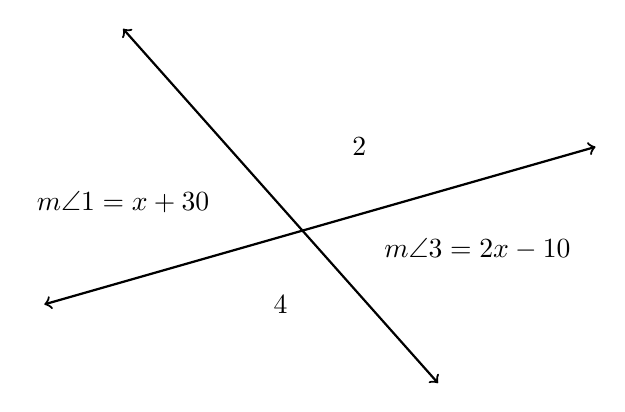
\begin{tikzpicture}[scale=1, rotate=0]
      \draw [<->, thick] (1,-1)--(8,1);
      \draw [<->, thick] (2,2.5)--(6,-2);
      \node at (2,.3){$m\angle 1= x+30$};
      \node at (6.5,-.3){$m\angle 3=2x-10$};
      \node at (5,1){2};
      \node at (4,-1){4};
      %\draw [fill] (0,0) circle [radius=0.05] node[below]{$P$};
      %\draw [fill] (6,0) circle [radius=0.05] node[below]{$R$};
      %\draw [fill] (3,0) circle [radius=0.05] node[below]{$Q$};
    \end{tikzpicture}
    \end{flushright}

\item Given $m\angle BAC = 5x-5$ and $m\angle DAC = x$, $m\angle BAD=115^\circ$. Find $m\angle BAC$.
  \begin{flushright}
  \begin{tikzpicture}[scale=1]
    \draw [<->, thick] (115:4)node[left]{$B$} 
    --(0,0)node[below]{$A$}
    --(10:5)node[below]{$D$};
    \draw [->, thick] (0,0)--(30:4)node[below right]{$C$};
    %\draw [fill] (0,0) circle [radius=0.05] node[below]{$A$};
    %\draw [fill] (5,0) circle [radius=0.05] node[below]{$B$};
  \end{tikzpicture}
  \end{flushright} \vspace{1cm}

\item An angle bisector is shown below, with $\overrightarrow{PR}$ bisecting $\angle QPS$. Given $m\angle QPR = 4x+2$ and $m\angle QPS = 10x-20$, find $m\angle QPS$.
    \begin{flushright}
    \begin{tikzpicture}[scale=0.6, rotate=30]
      \draw [<->, thick] (100:7)node[left]{$Q$} 
      --(0,0)node[below]{$P$}
      --(8,0)node[below]{$S$}--(9,0);
      \draw [->, thick] (0,0)--(50:7)node[below right]{$R$};
      %\draw [fill] (0,0) circle [radius=0.05] node[below]{$A$};
      %\draw [fill] (5,0) circle [radius=0.05] node[below]{$B$};
    \end{tikzpicture}
    \end{flushright}

\newpage   
  \subsubsection*{Do Not Solve! Make a drawing on the right, an equation to the left, and circle where it states what to find.}
  \vspace{0.5cm}

\item The point $Q$ is the midpoint of $\overline{PR}$, $PQ=11$, and $QR=2x+1$. Find ${x}$.
\vspace{4cm}

\item Given $\overline{PQR}$, with $PQ=3x-7$, $QR=x+3$, and $PR=12$. Find ${x}$.
\vspace{4cm}

\item Given that $Q$ bisects $\overline{PR}$. $PQ=2x-5$, $PR=42$. Find ${x}$.
\vspace{4cm}

\item The points $P$, $Q$, and $R$ are collinear, with $PQ=x+4$ and $PR=27$. $\overline{QR}$ is twice the length of $\overline{PQ}$. Find ${x}$.

\newpage
\subsubsection*{Do Not Solve! \\
Model the situation with an equation. Circle where it states what to find.}
\vspace{0.5cm}

\item Two lines intersect making four angles: $\angle 1$, $\angle 2$, $\angle 3$, and $\angle 4$. Given that $m\angle 1= 4x+30$ and $m\angle 2=8x-10$, find $x$.
\begin{flushright}
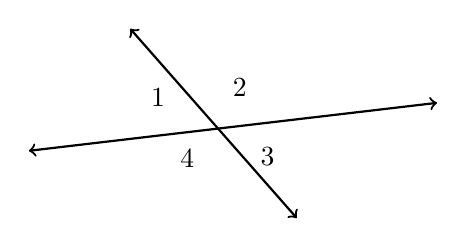
\begin{tikzpicture}[scale=0.5, rotate=-10]
\draw [<->, thick] (0,-1.5)--(10,1.5);
\draw [<->, thick] (2,2)--(7,-2);
\node at (3,.4){1};
\node at (6,-.6){3};
\node at (5,1){2};
\node at (4,-1){4};
\end{tikzpicture}
\end{flushright}

\item Given that $m\angle 2= 5x+30$ and $m\angle 4=7x-10$ as shown in the diagram, find $m\angle 2$.
\begin{flushright}
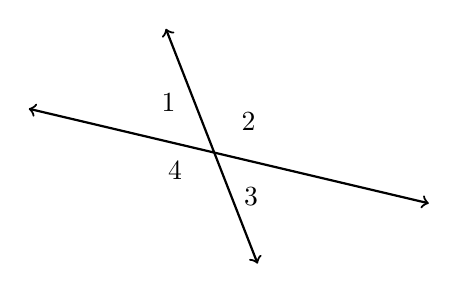
\begin{tikzpicture}[scale=0.5, rotate=-30]
\draw [<->, thick] (0,-1.5)--(10,1.5);
\draw [<->, thick] (2,2)--(7,-2);
\node at (3,.4){1};
\node at (6,-.6){3};
\node at (5,1){2};
\node at (4,-1){4};
\end{tikzpicture}
\end{flushright}

\item In the diagram below $\angle AOB = 30^\circ$ and $\angle COB = 5x+10$. Find $x$. \vspace{0.25cm}
\begin{flushright}
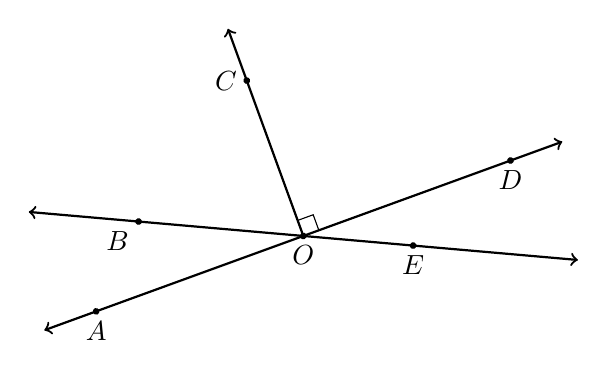
\begin{tikzpicture}[scale=0.7, rotate=20]
\draw [<->, thick] (-25:5)--(0,0)--(155:5);
\draw [<->, thick] (-5,0)--(5,0);
\draw [->, thick] (0,0)--(0,4);
\draw (0,0)++(0.3,0)--++(0,0.3)--+(-0.3,0);
%\draw [fill] (-1,2.5) circle [radius=0.05] node[left ]{$B$};
\draw [fill] (155:3) circle [radius=0.05] node[below left]{$B$};
\draw [fill] (-4,0) circle [radius=0.05] node[below]{$A$}; 
\draw [fill] (0,0) circle [radius=0.05] node[below]{$O$};
\draw [fill] (0,3) circle [radius=0.05] node[left]{$C$};
\draw [fill] (4,0) circle [radius=0.05] node[below]{$D$};
\draw [fill] (-25:2) circle [radius=0.05] node[below]{$E$};
\end{tikzpicture}
\end{flushright}

\item In the diagram below $\angle DOE = 60^\circ$ and $\angle DOB = 13x-10$. Find $x$. \vspace{0.25cm}
\begin{flushright}
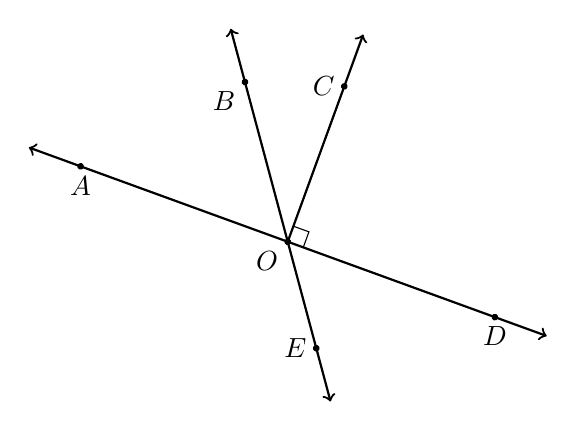
\begin{tikzpicture}[scale=0.7, rotate=-20]
\draw [<->, thick] (-55:3)--(0,0)--(125:4);
\draw [<->, thick] (-5,0)--(5,0);
\draw [->, thick] (0,0)--(0,4);
\draw (0,0)++(0.3,0)--++(0,0.3)--+(-0.3,0);
%\draw [fill] (-1,2.5) circle [radius=0.05] node[left ]{$B$};
\draw [fill] (125:3) circle [radius=0.05] node[below left]{$B$};
\draw [fill] (-4,0) circle [radius=0.05] node[below]{$A$}; 
\draw [fill] (0,0) circle [radius=0.05] node[below left]{$O$};
\draw [fill] (0,3) circle [radius=0.05] node[left]{$C$};
\draw [fill] (4,0) circle [radius=0.05] node[below]{$D$};
\draw [fill] (-55:2) circle [radius=0.05] node[left]{$E$};
\end{tikzpicture}
\end{flushright}


\end{enumerate}
\end{document}